\documentclass[oneside,12pt, draft]{fithesis2}  
\usepackage[czech]{babel}
\usepackage[utf8x]{inputenc} 
\usepackage[T1]{fontenc}  
\usepackage[plainpages=false,pdfpagelabels,unicode]{hyperref}  
%\usepackage{microtype}
\usepackage{fancyvrb}
\usepackage{url}
\usepackage{hyperref}
\usepackage{graphicx}
\usepackage[protrusion=true,expansion=true]{microtype}
\usepackage{cmap,tgpagella}

%\usepackage{cmap}	 % bod b) [do PDF bude přidáván potřebný font resource]
\usepackage[T1]{fontenc} % část bodu a) [vhodné kódování fontů]
\usepackage{lmodern}	 % část bodu a) [vhodný font]
\usepackage{listings}

 
\thesistitle{Relační přístup k~Amazon SimpleDB} 
\thesissubtitle{Diplomová práce}  
\thesisstudent{Radim Hopp}    
\thesiswoman{false}          
\thesisfaculty{fi}  
\thesisyear{2014}  
\thesisadvisor{doc. RNDr. Tomáš Pitner, Ph.D.}  
\thesislang{cs}            

\usepackage[plainpages=false,pdfpagelabels]{hyperref} 
\hyphenation{check-box}
\begin{document}  
\VerbatimFootnotes
\FrontMatter  
\ThesisTitlePage  

\setcounter{page}{1} 

\begin{ThesisDeclaration}  
\DeclarationText  
\AdvisorName  
\end{ThesisDeclaration}   

\begin{ThesisThanks}  
Rád bych poděkoval vedoucímu práce panu doc. Pitnerovi za ochotný přístup a věnovaný čas, dále také kolegům Filipovi Nguyenovi a Filipovi Eliášovi za vedení a směrování převážně v implementační části práce.
\end{ThesisThanks}  
 
\begin{ThesisAbstract}  
Cílem práce je prozkoumání možností relačního přístupu k NoSQL databázi Amazon SimpleDB, konkrétně mapování Teiid SQL dotazů na dotazy databáze Amazon SimpleDB. V rámci práce byl implementován fungující modul do projektu Teiid schopný základních CRUD operací nad databází SimpleDB. Dalším výstupem práce je tutoriál demonstrující instalaci, nastavení a základní použití vytvořeného modulu.
\end{ThesisAbstract}  
 
\begin{ThesisKeyWords}  
Amazon SimpleDB, JBoss Teiid, JBoss, databáze, relační přístup, NoSQL
\end{ThesisKeyWords}  
 
\MainMatter

\tableofcontents   
\chapter{Úvod}
Opensource projekt JBoss Teiid je silným nástrojem pro usnadnění a zkvalitnění práce aplikací nad více heterogenními zdroji dat. Aplikacím poskytuje jednotné rozhraní pro práci s daty a zajišťuje komunikaci s jednotlivými zdroji dat. 

Teiid již umí komunikovat s nejčastěji používanými zdroji dat, jakými jsou například relační databáze, LDAP či data uložena v souborech na disku. Bohužel ale nebyl prozatím vytvořen žádný modul do projektu Teiid pro komunikaci s NoSQL databází Amazon SimpleDB ikdyž po takovémto modulu byla poptávka už v roce 2010\footnote{V připomínkovacím systému JIRA projektu Teiid byl vytvořen požadavek už v dubnu 2010 -- https://issues.jboss.org/browse/TEIID-1070}. 

Jedním z důvodů, proč tento modul ještě nebyl vytvořen může být jeho netriviálnost. Jelikož je SimpleDB takzvanou NoSQL databází, což znamená, že nevychází z klasického modelu tabulek a relací mezi nimi, a jelikož Teiid ze své přirozenosti přistupuje k datům relačně, vyvstává zde několik možných problémů, které se tato práce snaží řešit.

Nejprve práce uvede čitatele do problému seznámením s projekty JBoss Teiid a Amazon SimpleDB, jejich fungováním, strukturou a fungováním.

Stěžejní částí teoretické práce je prezentace způsobu mapování Teiid SQL dotazů na dotazy a příkazy databáze Amazon SimpleDB. V této sekci nalezne čtenář řešení například absence schopnosti databáze SimpleDB spojit dvě tabulky (v SQL jde o klauzuli \texttt{JOIN}).

Praktická část práce detailně popisuje konkrétní implementaci modulů pro připojení a komunikaci s databází SimpleDB. 

Součástí práce je také tutoriál, který čtenáře provede instalací projektu Teiid, jeho základním nastavením pro použití s implementovaným modulem, připojením k databázi SimpleDB a provedením základních i komplikovanějších dotazů proti databázi pomocí projektu Teiid nad vzorovými daty. V textu práce je popsána struktura vzorových dat a zdůvodněna jejich volba.
% Následují další kapitoly a podkapitoly, popřípadě závěr, dodatky, 
% seznam literatury či použitých obrázků nebo tabulek.


\chapter{JBoss Teiid}

JBoss Teiid je otevřený software pro virtualizaci dat z~více zdrojů. Tento projekt je zaštiťován v~rámci JBoss komunitních projektů\footnote{http://www.jboss.org/overview/} spolu s~projekty jako WildFly nebo GateIn\footnote{kompletní seznam projektů na http://www.jboss.org/projects}.

Firma Red Hat nabízí také plně podporovanou a certifikovanou verzi pod názvem Red Hat JBoss Data Virtualization (dříve nazývaný Red Hat JBoss Enterprise Data Services Platform). Tento produkt kromě mírně upraveného komunitního projektu Teiid v~sobě obsahuje také JBoss Enterprise Application Platform (aplikační server založený na komunitním projektu WildFly) a další produkty\footnote{kompletní seznam produktů a projektů obsažených v~Red Hat JBoss Data Virtualization i s~použitými verzemi k~naleznutí na https://access.redhat.com/site/articles/703673}

\section{Systémy datové federace}
Datová federace úzce souvisí s datovou virtualizací (resp. je její specializací).
\begin{quotation}
 Datová virtualizace je pojem popisující jakýkoliv přístup k řízení dat, který umožňuje aplikaci získávat a manipulovat s daty bez znalosti technických detailů, jako třeba jak jsou formátována či kde jsou fyzicky uložena. \cite[volně přeloženo]{virtualizaceDat}
\end{quotation}
Takto definovaná virtualizace dat neříká nic o dílčích databázích či systémech, pouze říká, že existuje abstraktní vrstva, která zastiňuje strukturu, implementaci nebo třeba jazyk komunikace s databází. Takovouto vrstvou může být například aplikace komunikující s databází a vnějšku poskytující REST rozhraní. 

Datová federace poskytuje přístup k více heterogenním \textbf{autonomním} zdrojům dat. To znamená, že jednotlivým zdrojům dat je v nějaké míře zajištěna samostatnost (což v případě obecné virtualizace dat nemusela být pravda). Je to tedy forma virtualizace dat (je její specializací).

Software zajišťující manipulaci s dílčími databázovými systémy v rámci datové federace se nazývá \textbf{systém datové federace} (FDBMS - Federated database management system)\cite{fdbms}. Tento software by měl splňovat několik základních požadavků:
\begin{itemize}
 \item Virtualizace dat
 
 Jelikož je datová federace specializací datové virtualizace, měl by také software pro datovou federaci odstiňovat aplikace k němu přistupjící od implementačních, strukturních či jiných detailů jednotlivých databází a databázových systémů.
 
 \item Samostatnost dílčích systémů
 
 Oproti \uv{čisté} virtualizaci zaručuje systém datové federace jednotlivým databázovým systémům a zdrojům dat jistou autonomii. To znamená, že k jednotlivým podsystémům by se mělo dát přistupovat také samostatně, bez využití systému datové federace.
 
 \item Schopnost pracovat s heterogenními systémy
 
 Vedle autonomie jednotlivých subsytémů je dalším hlavním úkolem systémů datové federace schopnost komunikovat a pracovat s heterogenními systémy. Jednotlivé systému můžou být například soubory na disku, data přístupná z REST rozhraní či třeba SQL databáze. Je patrné, že ke každému z těchto datových systémů je nutné přistupovat různě. Zodpovědnost za správnou interpretaci dat nezávisle na schéma, implementaci, či rozdíly v datových typech jednotlivých systémů tak leží na bedrech systému datové federace.
\end{itemize} 

\section{JBoss Teiid a datová federace}


\section{Části projektu JBoss Teiid}
\begin{itemize}
 \item \textbf{Query engine}
 
 Jedná se o~srdce projektu, které zpracovává relační, XML, XQuery a jiné dotazy ze zdrojů dat. Také zajišťuje podporu pro schémata vytvořené z~jednoho, či z~více různých zdrojů dat. V~neposlední řadě se query engine stará o~transakce a uživatelem definované funkce.
 
 \item \textbf{JDBC ovladač}
 
 JDBC ovladač slouží pro jednoduché použití Teiidu v~externích java aplikacích.
 
 \item \textbf{Server}
 
 Tato část je zodpovědná za běh query enginu v~rámci aplikačního serveru (WildFly nebo Red Hat JBoss Enterprise Application Platform) a zaručuje škálovatelnost a snadnou správu. Součástí je administrační konzole, ve které je možno jednoduše nastavit například nasazenou virtuální databázi nebo nastavení vláken query enginu.

 \item \textbf{Konektory a překladače}

 Teiid přichází se~sadou konektorů a překladačů (connectors \& translators), díky kterým je schopen napojit se na řadu různých zdrojů dat. Konektory zajišťují napojení na zdroj dat, překladače potom obstarávají získávání dat podle Teiid požadavků. Základním kamenem jsou konektory pro většinu relačních databází, webové služby, textových souborů a LDAP\footnote{Lightweight Directory Access Protocol)}.
 
 Cíl této diplomové práce je rozšířit tuto sekci o~konektor pro NoSQL databázi Amazon SimpleDB.
 
 \item \textbf{Nástroje}
 
  \begin{itemize}
  \item Teiid Designer
  
  Teiid Designer je samostatný projekt (není součástí projektu JBoss Teiid), který ovšem také patří mezi komunitní projekty jboss.org. Jedná se o~sadu zásuvných modulů pro vývojové prostředí Eclipse, které mimo jiné usnadní vývoj virtuálních databází (pohledy, procedury, ...)
  
  \item Nástroje pro monitorování a správu
  
  Dvěmi hlavními nástroji pro monitorování a správu jsou Teiid Web Console (v~zásadě jde o~rozšíření webové konzole aplikačního serveru o~položky pro správu a monitorování Teiid instance) a zásuvný modul pro RHQ\footnote{RQH je komunitní projekt vedený pod jboss.org pro správu více serverů, http://www.jboss.org/rhq} pro kontrolu více serverů či clusterů Teiidu.
  
  \item Skriptování
  
  V~rámci Teiidu je také distribuován Teiid AdminShell, což je skriptovací nástroj založený na jazyku Groovy. AdminShell umožňuje spravovat Teiid z~příkazové řádky či pomocí skriptu, což uživateli velmi usnadní provádění často se opakujících činností.
  
  \end{itemize}

\end{itemize}

\chapter{Amazon SimpleDB}
SimpleDB je databáze z~dílen firmy Amazon a patří do skupiny produktů Amazon Web Services. Tato databáze je takzvaná NoSQL, což znamená, že data v~ní jsou uložená ve formátu, jaký není běžný pro relační databáze (tabulky, sloupce, řádky) a nepodporuje relace. SimpleDB je poskytována firmou Amazon jako služba a tudíž není možné nasadit databázi SimpleDB na vlastním serveru, ale běží pouze na serverech firmy Amazon. 
\section{Struktura databáze SimpleDB}
Strukturu SimpleDB databází je možno přirovnat k~tabulkovému procesoru.
\begin{itemize}
 \item \textbf{Uživatelský účet (Customer Account)}
 
 V~rámci jednoho účtu lze mít více domén stejně jako v~rámci jednoho souboru tabulkového procesoru je možno mít více listů s~tabulkami.
 \item \textbf{Doména (Domain)}
 
 Analogie k~jedné tabulce v~tabulkovém procesoru. Obsahuje řádky (položky), sloupce (atributy) a jednotlivé buňky (hodnoty).
 \item \textbf{Položky (Items)}
 
 Řádky tabulky. Reprezentují jednotlivé objekty uložené v~databázi s~jedním, či více vyplněnými atributy.
 \item \textbf{Atributy (Attributes)}
 
 Sloupce tabulky. Určují kategorie dat, jakých můžou položky nabývat.
 
 \item \textbf{Hodnoty (Values)}
 
 Hodnoty si lze představit jako jednotlivé buňky tabulky. Tady se ovšem analogie s~tabulkovým procesorem rozchází, neboť jedna \uv{buňka} může nabývat více hodnot najednou.
 
\end{itemize}
Navíc má každý prvek domény (řádek tabulky) povinný atribut \verb<ItemName<, který musí být v~dané doméně unikátní.

SimpleDB nepoužívá žádné jiné datové typy kromě typu \verb<String<, takže i čísla jsou v~databázi uloženy a je s~nimi nakládáno jako s~textovými řetězci. To s~sebou nese řadu problémů a hlavně zátěž na vývojáře aplikace tyto problémy řešit. Typickým příkladem takového problému je, že čísla nejdou řadit lexikograficky (lexikograficky: 10<2, což je špatně). Řešením je doplnění nul před čísla (00010>00002, což je správně).

\section{Vlastnosti databáze Amazon SimpleDB}
\subsection{SimpleDB jako služba}
Databáze Amazon SimpleDB je dodávaná jako služba. To znamená, že Amazon neposkytuje možnost nasadit tuto databázi ve vlastním prostředí, ale provozuje ji pouze na svých serverech. Uživatel databáze se tedy nemusí starat o~nastavování ani o~hardware, ale například ani o~škálování, nebo o~replikaci dat, jelikož Amazon automaticky distribuuje a synchronizuje data v~několika datových centrech umístěných v~různých geografických zónách, čímž omezuje nejen riziko ztráty dat, ale také zvyšuje rychlost přístupu k~datům v~různých místech na světě. Tím pádem se může uživatel databáze plně zaměřit na práci s~vlastními daty.
\subsection{Flexibilita}
Flexibilita je další z výhod databáze Amazon SimpleDB. Jelikož je to NoSQL databáze, není potřeba mít pevně dané schéma, jak tomu bývá u~SQL databází, ale nové atributy a entity mohou být přidávány takzvaně za pochodu.
\subsection{Indexování}
SimpleDB automaticky indexuje veškerá data v~ní uložené, čímž tato povinnost odpadá z~beder vývojářů aplikace a zvyšuje rychlost navracení výsledků čtecích operací.	
\subsection{Konzistence}
Amazon pro zápis zaručuje konzistenci takovou, že úspěšně provedený zápis (použitím příkazů jako např. \emph{PutAttributes}, \emph{BatchPutAttributes}, \emph{CreateDomain}, \dots) znamená, že všechny kopie databáze byly změněny. Toto pojetí konzistence ovšem nezaručuje chování při překrytí dvou či více zápisů najednou. Pouze zaručuje, že výsledné data budou na všech kopiích databáze rovná hodnotě jednoho z~těchto zápisů (toho, který databáze obdržela nejpozději). Toto bude níže ilustrováno na příkladě.
Při čtení si uživatel může zvolit mezi konzistentním a eventuálně konzistentním čtením. Konzistentní čtení zaručuje, že vrátí hodnotu po provedení posledního dosud přijatého zápisu. Eventuálně konzistentní čtení na druhou stranu vrátí hodnotu, která je aktuálně uložená na dotazovaném serveru (tj. může vrátit již neplatnou hodnotu).
\subsubsection*{Příklad konzistence}
Na obrázku \ref{consistencyExample} je uveden příklad, kdy se překrývají dva zápisy. V~této situaci není možné určit, jestli po provedení obou zápisů bude výsledná hodnota atributu \verb<Barva< rovna \verb<červená<, nebo \verb<zelená< z~toho důvodu, že není zaručeno, kterou instrukci zpracuje SimpleDB jako první. Například kvůli vysoké latenci sítě prvního klienta bude nejprve přijata a zpracována instrukce \verb<W2< druhého klienta a následně přepsána instrukcí \verb<W1<, tedy veškeré následné konzistentní čtení vrátí \verb<Barva=červená<.
\begin{figure}[h]
 \centering
 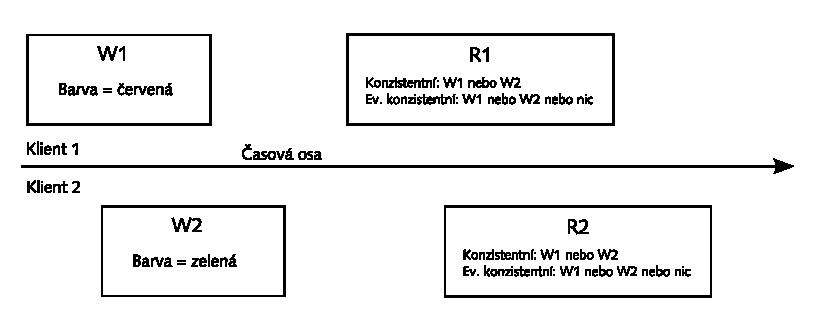
\includegraphics[scale=0.9]{ConsistencyExample}
 \caption{Ilustrace chování databáze SimpleDB}
 \label{consistencyExample}
\end{figure}

Jak bylo ukázáno, konzistentní čtení v~tomto případě mohlo vrátit jak výsledek \verb<W1<, tak výsledek \verb<W2<. Oproti tomu, výsledek eventuálně konzitentního čtení může být kromě \verb<W1< či \verb<W2< také \verb<nic<. Pravděpodobnost prázdného výsledku se s~časem minimalizuje, neboli čím déle po zápisu je čteno, tím větší je pravděpodobnost korektního výsledku.

%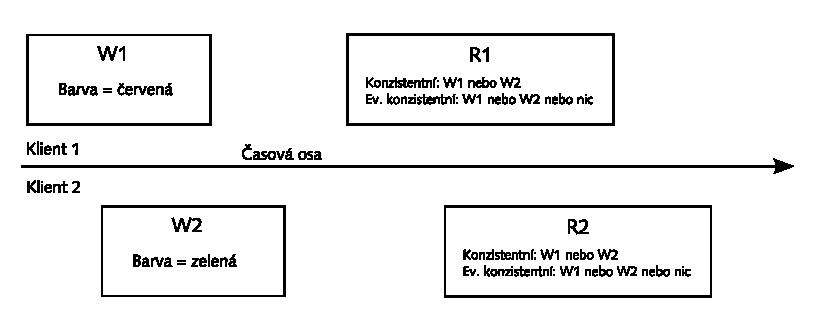
\includegraphics{ConsistencyExample}

Základní rozdíl mezi konzistentním a eventuálně konzistentním čtením lze shrnout do tabulky \ref{consistencyTable}
\begin{table}[h]
 \vspace{5mm}
 \begin{tabular}{l|l}
    Eventuálně konzistentní čtení & Konzistentní čtení\\ \hline
    Možné nekorektní výsledky & Vždy korektní výsledek\\ 
    Rychlejší odezva & Možná pomalejší odezva \\
    Větší datová propustnost & Možná menší datová prostupnost
 \end{tabular}
 \caption{Tabulka vlastností konzistentního a ev. konzistentního čtení}
 \label{consistencyTable}
\end{table}

\subsection{Omezení databáze SimpleDB}
Kromě výše zmíněného chování, které by se v~jistých situacích dalo považovat za omezení, je asi největším omezením velikost domény, jak co se místa na disku týče, tak také maximální počet atributů. Konkrétně je horní hranice 10 GB pro data a 1 miliarda atributů na jednu doménu. Domén je možno vytvořit až 250 na jeden uživatelský účet.


\chapter{Komunikace s~databází Amazon SimpleDB}
V této kapitole jsou popsány základní kameny komunikace s databází Amazon SimpleDB jako jsou například příkazy, zabezpečení či autentizace. Tyto poznatky jsou dále použity v implementační části (kapitola \ref{implementace})

\label{komunikace}
\section{Přehled příkazů SimpleDB}
\begin{itemize}
 \item \textbf{CreateDomain} slouží k~vytvoření nové domény.
 \item \textbf{DeleteDomain} vymaže danou doménu.
 \item \textbf{ListDomains} vrátí seznam domén asociovaných s~daným uživatelským účtem.
 \item \textbf{DomainMetadata} slouží k~získání informací o~doméně (datum vytvoření, počet položek v~doméně, počet atributů, \dots)
 \item \textbf{PutAttributes} vloží novou položku s~danými hotnotami atributů, či upraví již stávající položku.
 \item \textbf{Select} se podobá běžnému \verb<SELECT< příkazu, který je dobře známý z~SQL jazyků. Je ovšem mírně omezen a to například absencí \verb<JOIN< klauzule. Přesný přehled možností příkazu \verb<SELECT< databáze SimpleDB je uveden v~dokumentaci\footnote{http://awsdocs.s3.amazonaws.com/SDB/latest/sdb-dg.pdf}
 \item \textbf{GetAttributes} vrátí hodnoty požadovaných atributů jedné dané položky. Umožňuje specifikovat jeden, či více požadovaných atributů, nebo také všechny atributy dané položky.
\end{itemize}

\section{Podmíněné vkládání a mazání dat}
SimpleDB v~aktuální verzi (od 24. února 2010) podporuje takzvaný podmíněný zápis a mazání dat. 

Při tomto podmíněném zápise (mazání) se spolu s~běžnými parametry odešle také podmínka a očekávaný výsledek vyhodnocení dané podmínky. Zápis se poté provede pouze tehdy, je-li vyhodnocená podmínka rovna očekávanému výsledku.

Tato vlastnost se dá použít například pro implementaci čítače (přečte aktuální stav čítače a pokusí se zapsat nový stav čítače za podmínky, že stav čítače byl nezměněn), což by bez podmíněného vložení byl netriviální úkol. Také se tímto rozšiřují možnosti kontroly konkurenčního přístupu k~datům (pomocí optimistických protokolů \uv{optimistic concurrency control}).

\section{Bezpečnost}
Pro autentizaci má každý uživatel \uv{ID přístupového klíče} (20 alfanumerických znaků) a \uv{tajný přístupový klíč} (40 alfanumerických znaků), kterými podepisuje kažý požadavek vůči SimpleDB. Sama Amazon SimpleDB nemá nástroj pro autorizaci, ten je ovšem integrován do správy identit a přístupu AWS (AWS Identity and Access Management - systém pro správu uživatelů a jejich práv v~rámci celého AWS), takže je možné omezit práva jednotlivým uživatelům. Jediným problémem může být skutečnost, že nelze definovat přístupové práva pro jiný AWS účet -- pro každého uživatele domény musí být vytvořen uživatel v~rámci AWS účtu vlastnícího doménu.

\subsection{Proces autentizace}
\begin{enumerate}
 \item Vytvoření řetězce dotazu
 \item Kanonizování řetězce dotazu (seřazení parametrů, zakódování parametrů a jejich hodnot URL kódováním\footnote{Podle RFC 3986, kapitola 2 -- http://tools.ietf.org/html/rfc3986}), \dots)
 \item Vypočítání HMAC\footnote{Podle RFC 2104 -- http://www.ietf.org/rfc/rfc2104.txt} z~kanonizovaného textového řetězce za použití \uv{tajného přístupového klíče} jako klíče a SHA256 nebo SHA1 jako hashovacího algoritmu. Tento podpis se připojí k~původnímu požadavku jako parametr \verb<signature< spolu s~ID přístupového klíče jako \verb<AWSAccessKeyId<.
\end{enumerate}
Zde je ukázán proces autentizace pouze zjednodušeně. Přesný návod jak sestrojit validná požadavek je dostupný v~dokumentaci SimpleDB.

\section{Výběr knihovny pro komunikaci s databází SimpleDB}
Existují tři hlavní způsoby komunikace s databází SimpleDB v jazyce Java a to přímé volání REST API (popsaném v kapitole \ref{komunikace}), použití oficiálního Java API poskytovaného a podporovaného přímo společností Amazon nebo použití JDBC ovladače.

Nejprve se budu věnovat JDBC ovladači. Tento poměrně běžný a standartní způsob komunikace Java programů s databázemi by se mohl zdát jako nejlepší a nejjednodušší řešení. Toto tvrzení by podporoval i fakt, že jedna ze základních funkcionalit projektu Teiid je i konektor a překladač pro JDBC drivery. Lze tak \uv{podstrčit} projektu Teiid \verb&jar& soubor s JDBC ovladačem pro Amazon SimpleDB a vlastnostmi nutnými pro připojení (ID přístupového klíče a tajný přístupový klíč) a Teiid se již postará o vše ostatní. Hlavním argumentem proti použití JDBC ovladače je fakt, že se jedná o již prakticky mrtvý projekt\footnote{Webová stránka projektu: https://code.google.com/p/simpledb-jdbc/ a https://github.com/beacon50/SimpleJDBC}, který byl vyvíjen pouze jedním člověkem. O \uv{mrtvosti} projektu svědčí déle než  4 roky netknuté bugy v připomínkovacím systému (anglicky Issue tracker, dostupný na stránce projektu). Tento přístup také za ostatními dvěma alternativami zaostává na poli podpory. Kdežto Java API i REST API jsou podporovány přímo firmou Amazon, není zde, u JDBC ovladače, žádné záruky, že bude podporován do budoucna.

Tímto je zavrhnuto použití JDBC ovladače a zbývá rozhodnout, zda přistupovat k SimpleDB přímo pomocí volání REST API nebo pomocí Java API. Co se týče podpory, jsou na tom oba tyto přístupy stejně (oba oficiálně podporované firmou Amazon). V této práci bylo nakonec zvoleno Java API, převážně kvůli komfortu práce s kódem a následné čitelnosti kódu. Kdyby bylo použito přímé volání REST API, bylo by vhodné sepsat si vlastní Java API, což by zbytečně rozšiřovalo kódovou základnu projektu. Použití Java API z pohledu rozšíření kódu znamená pouze pár řádků v Maven konfiguraci, neboť je tato knihovna přítomna v Maven centrále\footnote{Detailně popsáno v kapitole \ref{sestaveni}}

\chapter{Mapování Teiid dotazů na SimpleDB dotazy}
V~této kapitole bude obecně ukázáno, jakým způsobem byly mapovány Teiid dotazy na dotazy databáze SimpleDB. Konkrétně se jedná o~příkazy \verb<SELECT<, \verb<INSERT<, \verb<UPDATE< a \verb<DELETE<.
\section{Vícehodnotové atributy}
Teiid přistupuje k~datům jako běžná relační databáze, tedy jednomu řádku a sloupci odpovídá nejvýše jedna hodnota. Z~tohoto důvodu je nutné ošetřit přístup k~vícehodnotovým atributům. Nabízí se několik řešení:
\begin{enumerate}
 \item Byl-li by dopředu znám maximální počet hodnot u~jednotlivých atributů, mohl by Teiid vnímat vícehodnotové atributy jako více sloupců tabulky (pro každou z~možných hodnot jeden sloupec). Tímto přístupem by se ovšem zafixovalo schéma a přišli bychom o~jednu z~hlavních výhod databáze SimpleDB (SimpleDB netrvá na pevném schématu).
 \item Zakódovat všechny hodnoty vícehodnotového atributu do jediného textového řetězce, který by byl lidsky i strojově čitelný. Tímto odpadá problém se změnou počtu hodnot atributu.
\end{enumerate}
Ve finální implementaci byl zvolen druhý přístup a hlouběji bude probrán v kapitole \ref{implementace}.

\section{SELECT}
Jelikož SimpleDB podporuje mírně omezený \verb|SELECT|, stačí vždy pouze poupravit řetězec příkazu \verb|SELECT| generovaný Teiidem, aby byl srozumitelný pro SimpleDB. Naštěstí lze pro každý překladač nadefinovat sadu podporovaných vlastností. Nepodporované vlastnosti obslouží sám Query Engine (např. překladač nepodporuje \verb<JOIN< klauzuli. Query Engine tedy rozloží dotaz s~\verb<JOIN< klauzulí na dva jednoduché dotazy, ty poté předá překladači a výsledné data zpracuje programově v~paměti).

Struktura příkazu SELECT databáze SimpleDB:
\begin{Verbatim}[frame=leftline,fontsize=\small]
select output_list
from domain_name
where [expression]
[sort_instructions]
limit [limit] 
\end{Verbatim}
Ze struktury je zřejmé, že žádné velké změny nebude třeba provádět. Je nutné definovat, že překladač nepodporuje \verb<JOIN< klauzuli a poté zajistit, aby byly korektně prováděny jednoduché SQL dotazy na které byl původní dotaz rozložen. Zde vyvstává pár problémů:
\begin{enumerate}
 \item Dotazu obsahujícímu atribut \verb<itemName()< (povinný unikátní atribut, který má každá položka) musí být tento atribut odebrán -- tento atribut je automaticky vracen v~odpovědi databáze ikdyž není specifikován. Naopak pokud je požadován spolu s~jinými atributy, databáze vrátí chybu. Toto platí s~výjimkou dotazu, kdy je \verb<itemName()< jediným požadovaným atributem.
 
 Tento dotaz je korektním dotazem na databázi SimpleDB a vrátí hodnoty atributu \verb<itemName()< všech položek v~doméně \verb<TestDomain<:
 \begin{Verbatim}[fontsize=\small]
SELECT itemName() FROM TestDomain
  \end{Verbatim}
 Tento dotaz vrátí chybovou hlášku \verb<InvalidQueryExpression<:
  \begin{Verbatim}[fontsize=\small]
SELECT itemName(), attribute1 FROM TestDomain
  \end{Verbatim}
 \item Další problém může vyvstat ve \texttt{WHERE} části výrazu. Těmto potížím se dá vyhnnout správným nastavením schopností překladače. 
\end{enumerate}

\section{INSERT}
Zde je situace stále celkem jednoduchá, neboť \verb<INSERT< vždy vkládá jeden nový řádek, což je téměř ekvivalentní příkazu \verb<PutAttributes<. Je zde akorát potřeba získat z~Teiid příkazu \verb<INSERT< seznam sloupců, jejich hodnot a název domény do které má proběhnout vložení. Vzhledem ke zvolenému řešení problému vícehodnotových atributů není nutné se jimi zaobírat zde (logika obsluhy vícehodnotových atributů je v implementaci extrahována do samostatného modulu).
\section{UPDATE}
U~\verb<UPDATE< je situace poněkud složitější, neboť je možné měnit více položek najednou (díky \verb<WHERE< klauzuli) a příkazy \verb<PutAttributes< a \verb<BatchPutAttributes< neumožňují měnit více položek specifikovaných pomocí kritéria najednou. Je tedy nutné nejprve pomocí \verb<SELECT< příkazu nad požadovanou doménou a kritérii z~Teiid \verb<UPDATE< dotazu získat jména všech upravovaných položek (atribut \verb<itemName()<). Teprve poté lze pomocí několika \verb<PutAttributes<, či jediného \verb<BatchPutAttributes< dané položky upravit.
\section{DELETE}
Podobně jako u~příkazu \verb<UPDATE< je nejprve potřeba získat jména všech položek, které mají být smazány a ty následně pomocí \verb<DeleteAttributes< smazat z~databáze.
\chapter{Implementace}
\label{implementace}
V~této kapitole bude rozebrána konkrétní implementace, problémy, které se během implementace vyskytly, a jejich řešení.
\section{Konektor}
Základním kamenem a prvním krokem v~implementaci bylo vytvoření konektoru.

Java EE Connector Architecture (JCA) je standardizované řešení pro připojení k~podnikovým informačním systémům (enterprise information systems). Stejně jako je JDBC zodpovědné pro připojení Java EE aplikací k~databázím, JCA je obecnější architektura pro připojení k~systémům, pro které není vytvořen JDBC ovladač. Základem každého konektoru je tzv. resource adapter, jež je odpovědný za přístup a interakci s~daným informačním systémem, který cheme připojit. Jednotlivé Java EE aplikace, nasazené v~aplikačním serveru, poté tento resource adapter využívají pro komunikaci. 

Specifikace JCA je vyvíjena v~rámci Java Community Process pod číslem JSR 322\footnote{Dostupné na webu Java Community Process -- http://www.jcp.org}
\subsection{Modul simpledb-api}
Tento modul reprezentuje API pro komunikaci s~databází SimpleDB a jako samostatný modul vzniknul hlavně kvůli oddělení závislostí na java knihovnu pro komunikaci se SimpleDB (aws-java-sdk) od ostatních modulů.

Modul obsahuje pouze jedinou java třídu a jedno rozhraní a to \texttt{SimpleDB\allowbreak APIClas} a \verb<SimpleDBConnection<.
\begin{itemize}
 \item \verb<SimpleDBConnection< je rozhraní rozšiřující rozhraní \verb<Connection< z~balíčku \verb<javax.resource.cci< (\verb<Connection< reprezentuje připojení na externí zdroj na aplikační vrstvě -- díky třídám implementující toto rozhraní je možné přistupovat k~požadovaným zdrojům).
 \item \verb<SimpleDBAPIClass< je třída zaobalující potřebné příkazy databáze SimpleDB. Za povšimnutí stojí hlavně metoda \texttt{Set<String> \\* getAttributeNames(String domainName)}, která vrací jména všech atributů v~doméně, ovšem jediný způsob jak toho docílit je provedení příkazu \texttt{SELECT * FROM <domainName>} a z~odpovědi získat jména všech atributů (nestačí dotázat se například na jednu položku, neboť kdyby daná položka neměla vyplněný nějaký atribut, tento atribut by v~odpovědi nebyl obsažen).
 
 Také je v této třídě obsažena veškerá logika manipulace s vícehodnotovými atributy.
\end{itemize}
\subsection{Modul connector-simpledb}
\label{connector-simpledb}
Jedná se o~plnohodnotný, ikdyž poměrně jednoduchý, Java EE konektor pro SimpleDB. Konektory jsou běžně baleny jako RAR (Resource Adapter Archive), které lze poté nasadit na aplikační server pouhým nakopírováním do složky \texttt{deploy} serveru. Teiid poskytuje základní implementaci rozhraní potřebných pro vytvoření zákadního konektoru. Zde bylo důležité uzpůsobit tuto základní implementaci potřebám databáze SimpleDB. 
\begin{itemize}
 \item Třída \texttt{SimpleDBManagedConnectionFactory} rozšiřuje abstraktní třídu \texttt{BasicManagedConnectionFactory} (základní Teiid implementace). V~této třídě je nutno definovat proměnné, které jsou potřebné pro připojení ke zdroji -- tedy proměnné ve kterých bude uložen ID přístupového klíče a tajný přístupový klíč spolu s~metodami pro jejich nastavení a získání (get a set metody). Požadované hodnoty budou aplikačním serverem získány z~konfiguračního souboru serveru (typicky třeba \texttt{standalone.xml}) a vloženy pomocí 
 \texttt{set} metod do těchto proměnných. Další důležitou částí je implementace abstraktní metody \texttt{creteConnectionFactory()}, pomocí které je vytvořena instance \texttt{ConnectionFactory}. Ta slouží ke~generování jednotlivých připojení ke zdroji dat (SimpleDB).
 
 \item Jako implementace rozhraní \texttt{Connection} zde slouží třída \texttt{SimpleDB\allowbreak ConnectionImpl}. Ta kromě implementování rozhraní \texttt{Connection} rozšiřuje základní Teiid implementaci \texttt{BasicConnection}. Nám zde tedy stačí zajistit přístup k~instanci třídy \texttt{SimpleDBAPIClass}. To je splněno instanciováním v~konstruktoru a přiřazením do privátní proměnné, která je poté dostupná pomocí její \texttt{get} metody.
 
 S~takto připraveným připojením lze poté v~samotném překladači snadno volat metody definované v~\texttt{SimpleDBAPIClass} např. takto:
 \begin{Verbatim}[fontsize=\small]
((SimpleDBConnectionImpl)connection).getAPIClass()
		.getDomains();
 \end{Verbatim}
 \item Dalším krokem je vytvoření konfiguračních souborů \texttt{MANIFEST.MF} a \texttt{ra.xml}. Oba soubory je nutno umístit do složky \texttt{META-INF}. 
 
 \texttt{MANIFEST.MF} obsahuje pouze závislosti resource adapteru. V~případě našeho konkrétního adapteru je to:
 \begin{Verbatim}[fontsize=\small]
Dependencies: org.jboss.teiid.common-core,
	    org.jboss.teiid.api,javax.api,
	    org.jboss.teiid.translator.simpledb.api
 \end{Verbatim}
 
 V~deployment descriptoru \texttt{ra.xml} definujeme hlavní třídu resource adapteru (tj. třída implementující rozhraní \texttt{Resource Adapter}), třídu implementující rozhraní \texttt{ManagedConnection\allowbreak Factory} a definujeme proměnné potřebné k~připojení k~SimpleDB (ID přístupového klíče a tajný klíč). 
 
 \item Celý tento modul je poté běžně zkompilován a balen jako Resource Adapter Archive -- RAR (běžný Java archive -- JAR s~příponou \texttt{.rar}), který může být nasazen na aplikační server zkopírováním do složky \texttt{deploy/}. Jelikož se zde ale nejedná o~konektor třetí strany, ale o~konektor, který bude dodáván s~projektem Teiid jako jeden ze základních konektorů, nestačí zajistit, že bude sestaven jako RAR, ale je potřeba, aby ve výsledku byl zařazen mezi moduly aplikačního serveru. K~tomu potřebné kroky budou popsány níže v~kapitole \ref{konfigurace} zabývající se kompilováním a sestavováním projektu pomocí projektu Apache Maven.
\end{itemize}

\section{Překladač}

Tento modul je rozdělen na tři logicky oddělené části. V~první je pouze třída \texttt{SimpleDBExecutionFactory}, která je základní třídou překladače. V~další části jsou zde takzvané executory -- třídy zajišťující vykonávání jednotlivých příkazů. Jako poslední jsou takzvané visitory -- třídy, které prochází strukturu Teiid SQL příkazu a získávají data, jež jsou poté použita v~executorech. Každá z~těchto částí je v~samostatném java balíčku.
\begin{figure}[h]
 \centering
 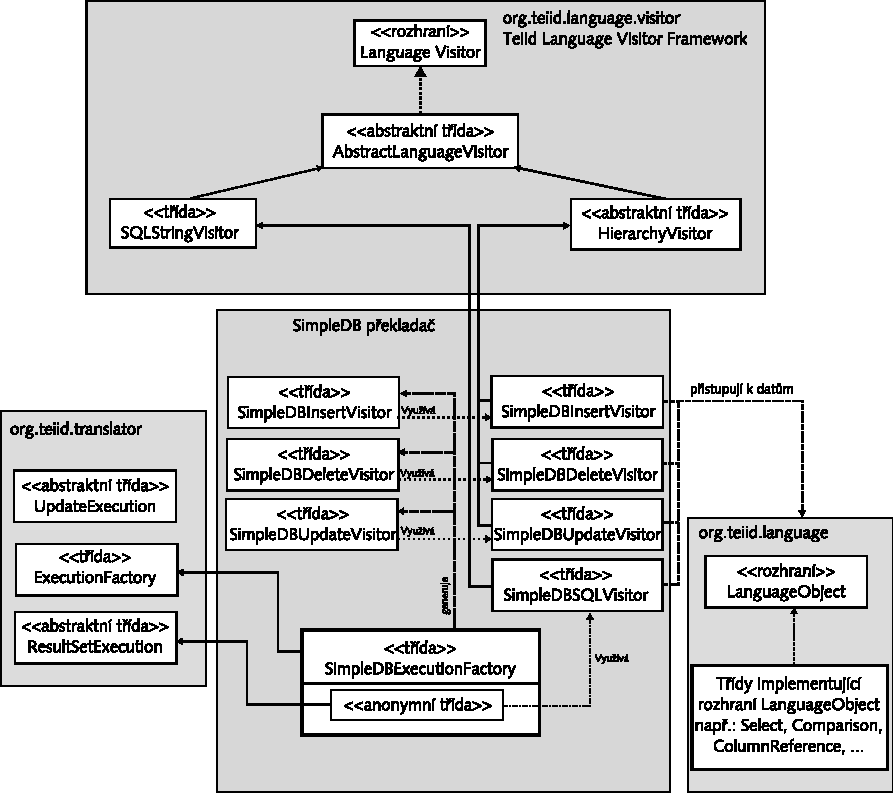
\includegraphics[scale=0.8]{TranslatorStructure}
 \caption{Struktura překladače SimpleDB}
\end{figure}
\subsection{SimpleDBExecutionFactory}
Základním kamenem SimpleDB překladače je třída \texttt{SimpleDBExecution Factory} rozšiřující abstraktní třídu \texttt{ExecutionFactory<F,C>}, kde \texttt{F} je factory třída konektoru a \texttt{C} je třída připojení -- v~našem případě se jedná o~\texttt{ConnectionFactory} a \texttt{SimpleDBConnection}.

Nejprve v~této třídě najdeme metody definující schopnosti překladače. Jedná se o~metody s~prefixem \texttt{supports} vracející boolean hodnotu podle toho zda překladač danou schopnost podporuje, či ne. Pro překladač SimpleDB byla zvolena tato množina podporovaných funkcí: 
\begin{verbatim}
supportsCompareCriteriaEquals
supportsCompareCriteriaOrdered
supportsInCriteria
supportsIsNullCriteria
supportsRowLimit
supportsNotCriteria
supportsOrCriteria
supportsLikeCriteria
\end{verbatim}
Zbylé funkce obstarává logika Teiidu.

Dále tato třída obsahuje metodu \texttt{void getMetadata(Metadata\allowbreak Factory metadataFactory, SimpleDBConnection conn)} (ukázaná na obrázku \ref{getMetadata}), kterou Teiid volá při inicializaci pro každou uživatelem definovanou virtuální databázi. Úkolem této metody je načíst strukturu databáze (tabulky, sloupce, typy, \dots) a pomocí \texttt{metadataFactory} ji předat Teiidu. Toho je docíleno iterací přes všechny domény a na nich voláním metody \texttt{getAttributeNames()} (metoda třídy \texttt{SimpleDBAPIClass} k~jejíž instanci lze přistupovat přes třídu implementující připojení -- \texttt{SimpleDB\allowbreak Connection}). Je nutné nastavit všem sloupcům datový typ \texttt{String} a také nezapomenout na atribut \texttt{itemName()}. Takto získané data poté stačí uložit do instance třídy \texttt{MetadataFactory}.

\begin{figure}[h]
 \begin{Verbatim}[fontsize=\small,numbers=left]
public void getMetadata(MetadataFactory metadataFactory, 
			SimpleDBConnection conn){
  List<String> domains = conn.getAPIClass().getDomains();
  for (String domain : domains) {
    Table table = metadataFactory.addTable(domain);
    table.setSupportsUpdate(true);
    Column itemName = new Column();
    itemName.setName("itemName()");
    itemName.setUpdatable(true);
    itemName.setNullType(NullType.No_Nulls);
    Map<String, Datatype> datatypes = metadataFactory
				      .getDataTypes();
    itemName.setDatatype(datatypes.get("String"));
    table.addColumn(itemName);
    for (String attrName : conn.getAPIClass()
			  .getAttributeNames(domain)) {
      Column column = new Column();
      column.setUpdatable(true);
      column.setName(attrName);
      column.setNullType(NullType.Nullable);
      column.setDatatype(datatypes.get("String"));
      table.addColumn(column);
    }
  }
}
 \end{Verbatim}
\label{getMetadata}
\caption{Ukázka metody getMetadata}
\end{figure}

Poslední dvě implementované metody v~této třídě jsou metody \texttt{createResultSetExecution} a \texttt{createUpdateExecution}, kde obě mají ve vstupních parametrech příkaz (\texttt{SELECT}, \texttt{UPDATE}, \dots), kontext, metadata a připojení. Obě tyto metody vrací instanci třídy implementující rozhraní \texttt{Execution}. Z~tohoto rozhraní je pro implementaci SimpleDB překladače nejdůležitější metoda \texttt{void execute()}, jejíž implementace je odpovědná za provádění konkrétního příkazu.

\begin{itemize}
 \item \texttt{createResultSetExecution}

Tato metoda je zodpovědná za veškeré příkazy určené k~získávání dat -- tedy primárně příkaz \texttt{SELECT}. Metoda
\texttt{createResultSet\allowbreak Execution} vrací nově vytvořenou anonymní třídu s~implementovanými metodami \texttt{void execute()} a \texttt{List<?> next()}. Metoda \texttt{execute} pouze pomocí třídy \texttt{SimpleDBSQLVisitor} získá seznam sloupců, poté pomocí stejné třídy získá textový řeťězec odpovídající příkazu \texttt{SELECT} a nad těmito daty zavolá metodu \texttt{performSelect} API třídy, která získá data z~databáze a vrátí je jako seznam. Ten je uložen do interní proměnne a v~metodě \texttt{next()} jsou tyto data pomocí iterátoru předávána Teiidu.

\item \texttt{createUpdateExecution}

Zde se obstarává vykonávaní všech metod manipulujících s~daty -- \texttt{INSERT}, \texttt{UPDATE}, \texttt{DELETE} a BatchedUpdate (který ovšem překladač simpledb nepodporuje).

Opět, podobně jako u~\texttt{createResultSetExecution} je zde potřeba vrátit třídu implementující rozhraní \texttt{UpdateExecution}, které se od \texttt{ResultSetExecution} liší pouze v~metodě získávání dat. Místo \texttt{List<?> next()} je zde \texttt{int[] getUpdateCounts()}. 
\end{itemize}
\subsection{Executory}
Jelikož je v metodě \texttt{createUpdateExecution} situace složitější než v metodě \texttt{createResultSetExecution} a řešení pomocí anonymní třídy by bylo velmi rozsáhlé, byla zde implementace rozdělena do 3 samostatných tříd podle příkazu, který zpracovávají -- \texttt{SimpleDBInsertExecute}, \texttt{SimpleDBDeleteExecute} a \texttt{SimpleDBUpdateExecute}.

Všechny tyto tři třídy využívají visitory (třídy vytvořené podle návrhového vzoru Visitor, budou popsány v kapitole \ref{visitory}) pro získání relevantních dat ze zadaného příkazu. 
\begin{itemize}
\item \texttt{SimpleDBInsertExecute} je nejjednodušší z~trojice executorů. Pouze pomocí \texttt{SimpleDBInsertVisitor} získá kolekci dvojic\\ \texttt{<jménoAtributu, hodnota\allowbreak Atributu>}, kde hodnota může být ve formátu \verb|^\[.+\]$|, což značí vícehodnotový atribut. Tuto kolekci poté předá metodě \texttt{perform Insert()} API třídy. O~správné zpracování vícehodnotových atributů se postará tato metoda.

\item \texttt{SimpleDBUpdateExecute} je opět poměrně jednoduchá třída -- mezivrstva mezi visitorem a API třídou vykonávající samotný dotaz na SimpleDB. Pomocí visitoru zjistí, které položky odpovídají porovnání v~dotazu. Přesněji řečeno získá hodnotu atributu \texttt{itemName()} všech položek odpovídajících podmínce \texttt{WHERE}. Dále zkonstruuje mapu map \texttt{Map<String, Map<String, String>} -- pro každý název položky získá pomocí visitoru \texttt{SimpleDBUpdate\allowbreak Visitor} mapu \texttt{<jménoAtributu, hodnotaAtributu>} a s~touto mapou map provede pomocí metody \texttt{performUpdate()} API třídy samotné upravení dat v~databázi.

\item V~případě \texttt{SimpleDBDeleteExecute} je zde pro jednoduchost a efektivnost rozděleno vykonávání do tří nezávislých větví podle situací, které mohou nastat:
\begin{itemize}
 \item Příkaz \texttt{DELETE} nemá klauzuli \texttt{WHERE}
 
  V~tomto případě executor rovnou pomocí API třídy zjistí hodnoty atributu \texttt{itemName()} všech položek v~dané doméně a tyto položky postupně pomocí metody \texttt{performDelete()} API třídy vymaže.
  
  \item Příkaz \texttt{DELETE} má klauzuli \texttt{WHERE} ve formátu \texttt{itemName() = <hodnota>}
  
  Zde se jedná o~jednoduché vymazání jediné položky. Tato položka je pomocí metody \texttt{performDelete()} vymazána.
  
\item Příkaz \texttt{DELETE} má klauzuli \texttt{WHERE} ve formátu jiném než \texttt{itemName() = <hodnota>}
  
  V~tomto případě je nutné nejprve zjistit hodnoty atributu \texttt{itemName()} položek, jež odpovídají podmínce klauzule \texttt{WHERE}. Tato logika je ponechána visitoru a zde se poté jen zavolá na získaných jménech metoda \texttt{performDelete()} API třídy.
\end{itemize}
\end{itemize}
Všechny tyto executory mají povinnost pamatovat si počet upravených, přidaných, či vymazaných řádků a tuto hodnotu zpřístupnit pomocí metody \texttt{int[] getUpdateCounts()}
\subsection{Visitory}
\label{visitory}
Tato sekce obsahuje 4 visitory. Každý ze 4 příkazů \texttt{SELECT, UPDATE, DELETE, INSERT} má jiné požadavky, proto pro každý z~nich byl vytvořen samostatný visitor.

Nejprve je ale třeba vysvětlit návrhový vzor Visitor, na kterém je celá tato sekce postavená.
\subsubsection*{Návrhový vzor Visitor}

Návrhový vzor visitor (někdy též návštěvník) je jedním ze základních návrhových vzorů popsaných již roku 1994 v~knize Design Patterns: Elements of Reusable Object-Oriented Software. Jedná se o~návrhový vzor, pomocí kterého je možné přidat skupině tříd dodatečnou funkcionalitu bez nutnosti změnit všechny tyto třídy. Také umožňuje funkcionalitu rozšířit za běhu programu.

V~tomto návrhovém vzoru jsou třídy rozdělené do dvou skupin -- navštěvované třídy a navštěvující třídy. Navštěvované třídy poskytují pouze základní funkcionalitu a navíc musí implementovat metodu, která příjme návštěvníka a předá mu data nutná k~jeho správnému fungování. Návštěvníci pro každou třídu, které chce rozšířit funkcionalitu, implementuje metodu \texttt{visit} se vstupním parametrem navštěvované třídy.


\subsubsection*{Jazykový visitor v~Teiidu}
Teiid disponuje rozhraním pro procházení a získávání dat ze stromů objektů jazyka založené na návrhovém vzoru visitor.

Každý Teiid příkaz je reprezentován stromem jazykových objektů -- tříd implementujících rozhraní \texttt{LanguageObject}. Toto rozhraní definuje jedinou metodu: 
\begin{Verbatim}[fontsize=\small]
void acceptVisitor(LanguageObjectVisitor visitor);
\end{Verbatim}
\texttt{LanguageObjectVisitor} je základní rozhraní pro všechny visitory a definuje \texttt{visit} metody pro všechny jazykové objekty jako například:
\begin{Verbatim}[fontsize=\small]
public void visit(AggregateFunction obj);
\end{Verbatim}
Teiid kromě základních rozhraní poskytuje i 3 základní implementace, kterých se dá využít při psaní vlastního visitoru:
\begin{itemize}
 \item \texttt{AbstractLanguageVisitor} je prázdnou implementací rozhraní \texttt{Language\allowbreak ObjectVisitor} poskytující nástroje pro procházení stromu jazykových objektů (sama ale žádné procházení nedělá). Tato třída není určena pro přímé použití, proto je definována jako abstraktní a je určena pouze pro použití jako rodičovská třída k rozšíření.
 \item \texttt{HierarchyVisitor} je podtřídou \texttt{AbstractLanguageVisitor} a je oproti její nadtřídě schopna projít všechny uzly stromu jazykových objektů. Nad těmito objekty ovšem neprovádí žádnou akci, pouze poskytuje jakýsi návod jak projít celý strom. Tato třída je také definována jako abstraktní a je určena k~rozšiřování.
 \item \texttt{DelegatingHierarchyVisitor} je rozšířením \texttt{HierarchyVisitor} o~možnost projít strom před a po projití hlavního visitoru. Tento nástroj není v~případě SimpleDB nutné využívat, proto se jím nebudeme zabývat dále.
 \item \texttt{SQLStringVisitor} je rozšířením základní abstraktní třídy \texttt{Abstract\allowbreak LanguageVisitor}, která dokáže daný objekt Teiid jazyka převést na textový řetězec řetězec odpovídající SQL příkazu.
 \item \texttt{CollectorVisitor} je třída vhodná pro získání všech objektů určitého typu z~jazykového stromu.
\end{itemize}

\subsubsection*{SimpleDBSQLVisitor}
\texttt{SimpleDBSQLVisitor} není v~této práci použit pouze pro příkaz \texttt{SELECT}, ale využívají jej i ostatní visitory pro získání jmen položek vyhovující podmínce. 

Jelikož má SimpleDB příkaz \texttt{SELECT} mírně odlišnou strukturu a nějaké omezení, nelze použít Teiidem dodávaný \texttt{SQLStringVisitor}, ale byla vytvořena tato třída.
\texttt{SimpleDBSQLVisitor} je rozšířením třídy \texttt{SQLStringVisitor} s~přetíženýma metodama \texttt{visit} pro objekty \texttt{Select, ColumnReference, Limit, Like a Comparison}.
\begin{itemize}
 \item \texttt{public void visit(Select obj)}
 
 Tato metoda je přetížena kvůli nutnosti odstranit atribut \texttt{itemName()} ze seznamu sloupců (\texttt{itemName()} je vracen automaticky a není třeba se na něj dotazovat)
 \item \texttt{public void visit(ColumnReference obj)}
 
 Implementace v~\texttt{SQLStringVisitor} vypisuje sloupec ve formátu \texttt{'tabulka'\allowbreak.'sloupec'}, což pro SimpleDB není žádoucí a je potřeba vypisovat sloupec bez tabulky.
 
 \item \texttt{public void visit(Comparison obj)}
 
 Jelikož Teiid podporuje operátor \texttt{NOT} (a v~\texttt{SimpleDBExecution\allowbreak Factory} bylo definováno, že náš překladač operátor \texttt{NOT} pdporuje), zdálo by se, že v~této oblasti je vše v~pořádku. Není tomu ovšem tak, neboť ve chvíli, kdy překladač podporuje \texttt{NOT} operátor, zaručuje také podporu negovaných operátorů. Jedním z~těchto negovaných operátorů je operátor \uv{nerovná se -- <>}, a jelikož jej databáze SimpleDB nepodporuje, musí být při generování SQL řetězce převeden na \uv{NOT =}
 \begin{Verbatim}[fontsize=\small,numbers=left]
if (obj.getOperator().equals(Operator.NE)){
  Comparison c = new Comparison(obj.getLeftExpression(), 
		obj.getRightExpression(), Operator.EQ);
  append(new Not(c));
}
 \end{Verbatim}
\item Další změny jsou pouze minoritního charakteru.
\end{itemize}

\subsubsection*{SimpleDBInsertVisitor}
Vše co je potřeba na vykonání SimpleDB příkazu \texttt{PutAttributes} je jméno domény a mapa jména atributu a hodnot atributů. To je zajištěno rozšířením abstraktní třídy \texttt{HierarchyVisitor} a přetížením jeho \texttt{visit} metod pro parametry typu \texttt{ColumnReference} a \texttt{ExpressionValueSource}.

Při návštěvě \texttt{ColumnReference} (sloupců) se tvoří seznam názvů sloupců. Poté se při návštěvě \texttt{ExpressionValueSource} (ekvivalent klauzuli \texttt{VALUES}) tvoří mapa, kde jako klíč poslouží jméno atributu a jako hodnota hodnota atributu. Jelikož \texttt{HierarchyVisitor} prochází pomyslný strom Teiid příkazu do hloubky, je zajištěno, že seznam jmen atributů bude sestaven před začátkem zpracovávání vkládaných hodnot.

Pro získání těchto hodnot je implementována statická metoda \texttt{get\allowbreak Columns\allowbreak ValuesMap(Insert insert)}, ta instanciuje vlastní třídu předá ji objektu \texttt{Insert} jako návštěvníka, který ji projde. Následně vrátí získané hodnoty.

\subsubsection*{SimpleDBUpdateVisitor}
Ikdyž je i tento visitor založen na \texttt{HierarchyVisitor} je zde situace poněkud složitější, než v~případě \texttt{SimpleDBInsertVisitor} a to hlavně protože pokud v~příkazu existuje podmínka, je nutné zjistit jména všech položek odpovídajících podmínce. Proto je zde zvolen jiný přístup, než u~\texttt{SimpleDBInsertVisitor} (statické třídy pro získávání dat). Zde je navštěvování položek příkazu spuštěno v~konstruktoru, tedy při vytvoření instance, a následně lze \texttt{get} metodami získat \uv{vydolované} data.

Konstruktor je parametrický a kromě instance \texttt{Update} přijímá i instanci připojení a to z~kvůli možné podmínce (je potom potřeba dotázat se databáze na jména položek vyhovující podmínce).

Požadované data zde jsou: název domény, mapa jmen atributů a jejich hodnot a seznam jmen položek odpovídajících podmínce.

Přetížené metody \texttt{visit} jsou pro objekty typu \texttt{Update}, \texttt{SetClause} a \texttt{Comparison}

\begin{itemize}
 \item \texttt{Update} kromě implicitního zavolání metod \texttt{visit} pro objekty níže ve stromu příkazu (\texttt{SetClause, Condition}) si také uloží jméno domény do privátní proměnné.
 \item \texttt{SetClause} vytvoří a naplní mapu jmen atributů a jejich hodnot.
 \item Hlavním úkolem metody \texttt{visit(Comparison obj)} je získání hodnot atributu \texttt{itemName()} všech položek vyhovující podmínce. To lze jednoduše zajistit \texttt{SELECT} dotazem přímo na databázi SimpleDB, kde se do \texttt{WHERE} klauzule vloží řetězec vygenerovaný pomocí \texttt{SimpleDBSQLVisitoru} pro danou podmínku, jak je vidět v~následující ukázce kódu na řácích 4-6. Na řádcích 7-8 pak pouze probíhá uložení získaných jmen položek do privátní proměnné \texttt{itemNames}.
 \begin{Verbatim}[fontsize=\small,numbers=left]
public void visit(Comparison obj) {
  ArrayList<String> columns = new ArrayList<String>();
  columns.add("itemName()");
  List<List<String>> response = apiClass.performSelect("SELECT "
      +"itemName() FROM "+tableName+" WHERE "+SimpleDBSQLVisitor
      .getSQLString(obj), columns);
  for (List<String> list : response) {
    itemNames.add(list.get(0));
  }
}
 \end{Verbatim}
\end{itemize}

\subsubsection*{SimpleDBDeleteVisitor}
Zde je použit stejný přístup jako u~\texttt{SimpleDBUpdateVisitor}. Tedy spuštění procházení stromu v~parametrickém konstruktoru, který kromě instance navštěvovaného objektu přijímá také API třídu \texttt{SimpleDBAPIClass} potřebnou pro komunikaci se SimpleDB.

Je zde potřeba rozlišovat mezi třemi základními situacemi:
\begin{itemize}
 \item Žádná \texttt{WHERE} klauzule -- tato situace je vyřešena již v~executoru \texttt{SimpleDBDeleteExecute} dotázáním na existenci této klauzule a případným smazáním všech záznamů z~domény.
 \item V~klauzuli \texttt{WHERE} je jednoduchá podmínka tvaru \texttt{itemName() = <hodnota>} nebo \texttt{<hodnota> = itemName()}. V~tomto případě je nastavena hodnota privátní proměnné \texttt{boolean isSimpleDelete} na \texttt{true}. Na tuto proměnnou se poté dotazuje \texttt{SimpleDBDelete\allowbreak Execute} a zařizuje se podle ní.
 \item Posledním případem je složitější podmínka ve \texttt{WHERE} klauzuli. V~tomto případě se \texttt{SimpleDBDeleteVisitor} chová téměř totožně jako \texttt{SimpleDBUpdateVisitor} a to tak, že se nejprve dotáže databáze SimpleDB jednoduchým \texttt{SELECT} příkazem s~\texttt{WHERE} klauzulí daného \texttt{DELETE} příkazu (vygenerovanou pomocí \texttt{SimpleDBSQL\allowbreak Visitor}).
\end{itemize}
\section{Sestavení}
\label{sestaveni}
Pro kompilaci a sestavení celého projektu je použit projekt Apache Maven. Maven kromě usnadnění a zautomatizování procesu sestavení také obstarává správu závislostí. Schopnosti mavenu je dále možné rozšířit pomocí zásuvných modulů (plug-inů).
\begin{figure}[h]
 \centering
 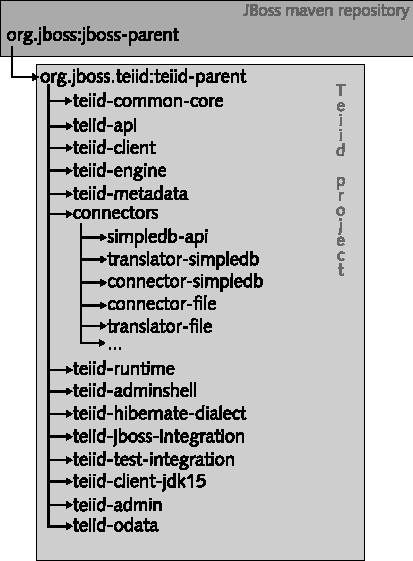
\includegraphics[scale=1]{mavenStructure}
 \caption{Maven struktura projektu Teiid}
\end{figure}

Projekt Teiid je rozdělen do takzvaných modulů. Moduly jsou jednotlivé logické celky vytvořené jako java projekty. Každý takový modul má svůj soubor pom.xml (Project Object Model) -- konfigurační soubor projektu. V~tomto souboru jsou definovány identifikátory projektu (ID artefaktu, ID skupiny, verze, ...), identifikátory rodičovského POM souboru, závislostí a konfigurací použítých maven zásuvných modulů.

\subsection{Konfigurace jednotlivých SimpleDB modulů}
\label{konfigurace}
\begin{itemize}
 \item \textbf{simpledb-api}
 
 Zde není potřeba žádné speciální konfigurace. Stačí definovat v~pom.xml závislosti, rodičovské pom.xml a v~rodičovském pom.xml definovat tento projekt jako modul (přidat do tagu \texttt{<modules>}).
 \item \textbf{connector-simpledb}
 
 Tento modul má na konfiguraci zvláštní požadavky, neboť musí být sestaven jako rar archiv a následně nainstalován do lokálního repozitáře, aby pak byl dostupný v~poslední fázi sestavení kompletního projektu Teiid.
 
 Potřebné soubory \texttt{MANIFEST.MF} a \texttt{ra.xml} byly popsány již v~kapitole \ref{connector-simpledb}, zbývá tedy nastavit Maven pomocí pom.xml.
 K~sestavení projektu jako \texttt{rar} je použit zásuvný modul \texttt{maven-rar-plugin} spuštěný v~rámci maven fáze \texttt{install}. Toto vytvoří korektní \texttt{rar} archiv a následně (stále ve fázi \texttt{install}) je pomocí zásuvného modulu \texttt{maven-install-plugin} tento soubor nainstalován do lokálního maven repozitáře, aby byl přístupný i ostatním projektům.
 
 \item \textbf{translator-simpledb}
 
 Překladač nevyžaduje žádné speciální nastavení. Stačilo tedy zajistit, aby v~souboru \texttt{pom.xml} byl definován správný rodič (\texttt{org.jboss.teiid:connectors}) a v~rodiči byl projekt \texttt{translator\allowbreak -simpledb} registrován jako modul.
\end{itemize}

\subsection{Nastavení zásuvného modulu maven assembly plugin}
Projekt Teiid je dodáván v~distribucích \texttt{Teiid Runtime} nebo \texttt{Teiid Embedded}. Další dodávané produkty jsou JDBC ovladač a Teiid Admin Shell. 

\texttt{Teiid Runtime} je Teiid připravený k~okamžitému nasazení na aplikační server WildFly (verze 8 a vyšší), nebo Red Hat JBoss Enterprise Application Platform (verze 6.1 a vyšší). Obsahuje v~sobě kromě zkompilovaných knihoven, modulů a dokumentace také výchozí konfigurační soubory včetně \texttt{standalone.xml}.

\texttt{Teiid Embedded} je odlehčená verze Teiidu pro použití bez aplikačního serveru, schopna běžet jako samostatná java aplikace. Tímto bohužel přichází o~vlastnosti jako například autentizace, přístup přes administrační rozhraní  nebo správu připojení (connection pooling).

Sestavení těchto distribucí ze zkompilovaných artefaktů do finálních \texttt{.zip} souborů má na starosti Maven Assembly Plugin. 

Z~pohledu SimpleDB konektoru a překladače bylo potřeba zajistit 3 věci:

\begin{itemize}
 \item Upravit kostru konfiguračního souboru aplikačního serveru. To znamená přidat do souboru \texttt{standalone-teiid.xml} definici resource adapteru konektoru SimpleDB a zajistit, aby překladač byl uveden v~subsystému teiidu.
 \item Vytvořit konfigurační soubory modulů (\texttt{module descriptor}) pro každý modul překladače simpledb (api, konektor, překladač)
 \item Upravit konfigurační soubor, podle kterého zásuvný modul maven assembly zkompletuje výsledné \texttt{.zip} soubory. Níže je výňatek z~tohoto konfiguačního souboru (tzv. assembly descriptor). V~tomto konkrétním případě se jedná o~instalaci artefaktu \texttt{simpledb-api} jako modulu aplikačního serveru JBoss AS (jak je vidět na řádcích 21-22):
 \begin{Verbatim}[fontsize=\small,numbers=left]
...
<moduleSet>
  <includeSubModules>true</includeSubModules>
  <useAllReactorProjects>true</useAllReactorProjects>
  <includes>
      <include>org.jboss.teiid.connectors:simpledb-api</include>
  </includes>
  <binaries>        
    <includeDependencies>true</includeDependencies>
    <unpack>false</unpack>
      <dependencySets>
	  <dependencySet>
	      <useProjectArtifact>true</useProjectArtifact>
	      <unpack>false</unpack>
	      <useTransitiveDependencies>
		false
	      </useTransitiveDependencies>
	      <useDefaultExcludes>true</useDefaultExcludes>
	  </dependencySet>
      </dependencySets>          
    <outputDirectory>modules/system/layers/base/org/jboss/
	      teiid/translator/simpledb/api/main</outputDirectory>
    <fileMode>0644</fileMode>
  </binaries>
</moduleSet>  
...
\end{Verbatim}
    
\end{itemize}



\chapter{Quickstart}
Jelikož se SimpleDB profiluje jako velmi rychlá, velmi dobře škálovatelná databáze s~omezeními co se týče struktury, velikosti dat a konzistence, je její nasazení vhodné v~prostředích:
\begin{itemize}
 \item Kde je poměr čtení-zápis výrazně ve prospěch čtení -- čte se často a je požadována rychlost odpovědi, zapisuje se zřídka (kvůli konzistenci)
 \item Kde je kladen vysoký důraz na rychlost čtení i na úkor konzistence (přístup \uv{nevadí, že nedostanu aktuální výsledek, hlavně když jej dostanu rychle})
\end{itemize}
Běžný přístup ve firemním prostředí je nasazení SimpleDB jako doplňkové databáze ke klasické relační databázi. V~této situaci mohou být v~SimpleDB uložena například metadata, případně často čtené položky.

Inspirací pro zdrojová data pro tutoriál byla firma Netflix. Netflix je firma živící se převážně streamováním filmů a seriálů a pro správu dat zvolil řešení firmy Amazon. Mezi jinými tedy i databázi SimpleDB\footnote{http://techblog.netflix.com/search/label/SimpleDB}.

V~rámci této diplomové práce byl jako zdroj dat zvolen \texttt{.csv} soubor s~daty o~filmech vydaných v~lednu roku 2013. Soubor obsahuje:
\begin{itemize}
 \item Název filmu
 \item Studio ve kterém byl film natočen (může se jednat o~více studií)
 \item Režisér a herecké obsazení (zde se jedná o~čárkami oddělené jména)
 \item Žánr filmu (žánrů může být více)
 \item Box office, aneb kolik dolarů daný film vydělal.
\end{itemize}
Na obrázku \ref{relationStructure} je znázorněno, jakou strukturu by měla klasická relační databáze pro výše zmíněné data. 
\begin{figure}[h]
 \centering
 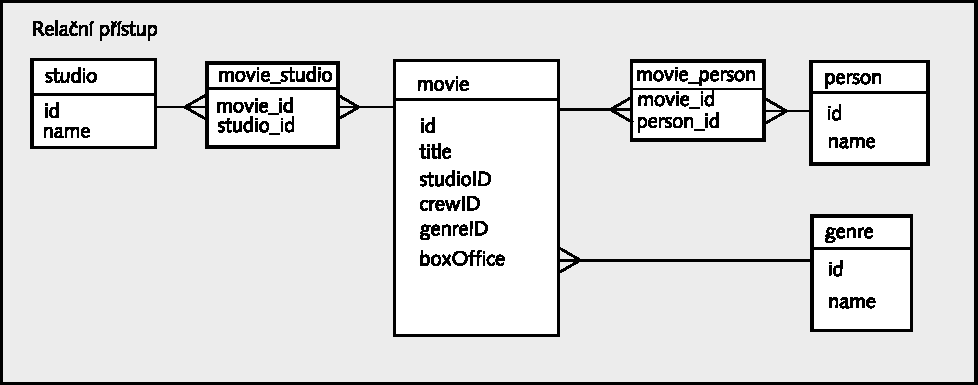
\includegraphics[scale=0.8]{relationStructure}
 \caption{Struktura uložení dat v~relační databázi}
 \label{relationStructure}
\end{figure}

Na druhou stranu obrázek \ref{simpledbStructure} ukazuje jak by s~velkou pravděpodobností byla uložena data v~databázi SimpleDB. Normalizace databáze zde nehraje roli, duplikáty nejsou na škodu. Je zde kladen důraz na jednoduchost a rychlost.
\begin{figure}[h]
 \centering
 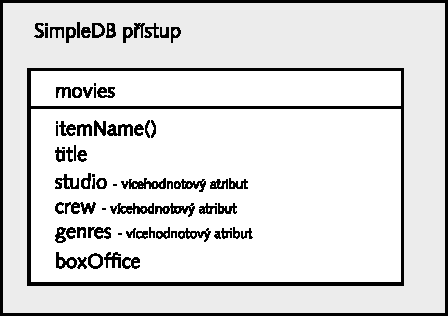
\includegraphics[scale=0.8]{simpledbStructure}
 \caption{Struktura uložení dat v~databázi SimpleDB}
 \label{simpledbStructure}
\end{figure}

Aby byly ukázány aspekty obou přístupů -- jak relačního, tak přístupu z~pohledu SimpleDB -- jsou vzorová data uloženy v~databázi se strukturou ukázanou na obrázku \ref{kompromisStructure}. Takto bude možnost demonstrovat například schopnost spojování výsledků ze dvou a více vstupních množin (klauzule \texttt{JOIN} -- jedna ze základních schpností relačních databází, která databáze SimpleDB nepodporuje), nebo schopnost pracovat s~vícehodnotovými atributy (což je výsadou databáze SimpleDB oproti relačním databázím).

\begin{figure}[h]
 \centering
 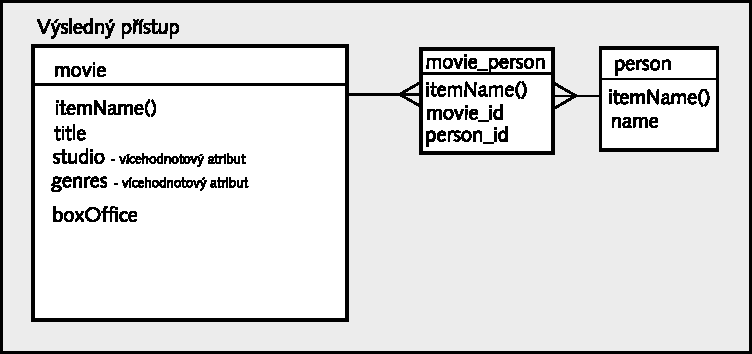
\includegraphics[scale=0.8]{kompromisStructure}
 \caption{Výsledná (kompromisní) struktura databáze}
 \label{kompromisStructure}
\end{figure}
\vspace{30mm}
V~rámci přípravy tutoriálu byl vytvořen java program \texttt{impotData}, který dokáže umístit vzorové data do uživatelovy instance databáze SimpleDB. Pro snadné použití byl projekt mavenizován a pro snadnou dostupnost byl spolu s~tutoriálem umístěn na server GitHub, který je určen k~hostování a verzování projektů pomoví verzovacího systému Git.

Do stejného repozitáře byl také umístěn soubor \texttt{README.md} (formátovaný pomocí Markdown) obsahující vlastní tutoriál, který uživatele provede (v anglickém jazyce) nainstalováním Teiidu, vytvořením virtuální databáze, připojením k lokálně běžící instanci Teiidu a několika vzorovými dotazy na SimpleDB pomocí JDBC ovladače Teiidu.

Příloha A je pouze tutoriál převedený z Markdown do latexu. Originální Markdown soubor je v GitHub repozitáři, nebo na přiloženém CD.
\chapter{Závěr}
Výsledkem práce je funkční konektor (resource adapter) pro připojení k SimpleDB. Dále byl vytvořen modul Teiid překladače (translator) pro SimpleDB ve kterém se povedlo zvládnout problematiku mapování Teiid SQL dotazů na dotazy databáze SimpleDB. Také zde byl úspěšně řešen problém multihodnotových atributů databáze SimpleDB. Tyto části dohromady tvoří funkční modul projektu Teiid a již byly zařazeny do hlavní vývojové větve projektu. Teiid 8.7 již v sobě bude obsahovat modul pro komunikaci s databází SimpleDB vytvořený v rámci této práce.

Druhým výstupem je tutoriál v anglickém jazyce, hostovaný veřejně na serveru GitHub, který slouží jako uvedení do problematiky pro nové uživatele a demonstruje schopnosti vyvinutého Teiid modulu.

Tato práce pro mě znamenala jedny z prvních krůčků do světa open-source a velkou zkušeností pro mě byla spolupráce s lidmi, kteří programují otevřený software, jelikož bych se otevřeným softwarem rád zabýval i v budoucnu.

Dalším krokem ve vývoji Teiid modulu pro komunikaci se SimpleDB by bylo zaměření se na výkon -- sepsání \uv{performance testů} a optimalizace kódu. Také je možnost pokusit se začlenit tutoriál vyvinutý v rámci této práce mezi oficiální \uv{quickstarty}\footnote{https://github.com/teiid/teiid-quickstarts}.
\nocite{*}
\bibliographystyle{plain}  % bibliografický styl 
\bibliography{mybib} % soubor s citovanými
                           % položkami bibliografie 

\appendix
\chapter{Tutoriál}
\section*{This is quickstart for SimpleDB connector and translator for Teiid - https://github.com/teiid/teiid}
\subsection*{System Requirements}
To run this quickstart with the provided build scripts, you need the following:
\begin{enumerate}
 \item Java 1.6 or better, to run JBoss AS and Maven. You can choose from the following:
 \begin{itemize}
  \item OpenJDK
  \item Oracle Java SE
  \item Oracle JRockit
 \end{itemize}

 \item Maven 3.0.0 or newer, to build and deploy the example
 \begin{itemize}
  \item If you have not yet installed Maven, see the Maven Getting Started\footnote{http://maven.apache.org/guides/getting-started/index.html} Guide for details.
  \item If you have installed Maven, you can check the version by typing the following in a command line:

  \texttt{mvn --version}
 \end{itemize}
 
 \item The JBoss Enterprise Application Platform (EAP) 6.1 (and higher) distribution ZIP or the JBoss AS 7.2 (or WildFly 8 or higher) distribution ZIP.
 \begin{itemize}
  \item For information on how to install and run JBoss, refer to the server documentation.
 \end{itemize}

 \item Amazon AWS credentials
 \begin{itemize}
  \item If you don't have one, go to aws.amazon.com and sing up for using Amazon SimpleDB
  \item Your access credentials can be found on https://portal.aws\allowbreak .amazon.com/gp/aws/securityCredentials
 \end{itemize}

 \item Client for executing queries against Teiid
 \begin{itemize}
  \item Some JDBC client. This is preferred variant. This example will be demonstrated using Squirrel SQL client - http://squirrel-sql.sourceforge.net/
  \item Some tool for executing querries directly to Teiid. For example simpleclient from teiid-quickstarts github repository - https://github.com/teiid/teiid-quickstarts
 \end{itemize}
\end{enumerate}


\subsection*{Installing Teiid}
Project Teiid (version 8.6) is compatible with EAP 6.1 or WildFly 8\footnote{As SimpleDB support will be in Teiid since version 8.7 (and 8.7 is not out yet) you may need to compile teiid from source code as described in here: https://community.jboss.org/wiki/TeiidEclipseDevEnvironmentSetUpAndBuildingRuntimeArtifacts}.

\begin{enumerate}
 \item Install application server (by uncompressing it to desired folder)
 \item Download latest Teiid Runtime from http://www.jboss.org/teiid/downloads and install it
 \begin{itemize}
  \item Installing teiid is just matter of extracting into WildFly or EAP directory.
 \end{itemize}
 \item Add connection definition to resource adapter
 \begin{itemize}
  \item Open \texttt{\$AS\_ROOT\_DIRECTORY/standalone/configuration/\allowbreak standalone-teiid.xml} in your favourite text editor
  \item Add this snippet under simpledb resource adapter to look like so (do not forget to fill your access key id \& access key):
  \begin{Verbatim}[fontsize=\small]
<resource-adapter id="simpledb">
  <module slot="main" 
  id="org.jboss.teiid.resource-adapter.simpledb"/>
  <connection-definitions>
      <connection-definition 
      class-name="org.teiid.resource.adapter.simpledb.
		  SimpleDBManagedConnectionFactory" 
      jndi-name="java:/simpledb" enabled="true" 
      use-java-context="true" pool-name="fileDS">
	  <config-property name="AccessKey">
	      <YOUR_ACCESS_KEY_ID>
	  </config-property>
	  <config-property name="SecretAccessKey">
	      <YOUR_SECRET_ACCESS_KEY>
	  </config-property>
      </connection-definition>
  </connection-definitions>
</resource-adapter>
  \end{Verbatim}
 \item Create virtual database file (VDB) and deploy it:
 \begin{itemize}
  \item Create file \texttt{my-vdb.vdb} with content:
  \begin{Verbatim}[fontsize=\small]
<?xml version="1.0" encoding="UTF-8" standalone="yes"?>
<vdb name="Test" version="1">

<description>Test</description>
<model name="Test">
    <source name="simpledb-connector" 
	  translator-name="simpledb" 
	  connection-jndi-name="java:/simpledb"/>
</model>
</vdb>   
  \end{Verbatim}
 \item Save this file to your AS deploy folder (\texttt{\$AS\_ROOT\_DIRECTORY/\allowbreak standalone/deployments/my-vdb.vdb})
 \end{itemize}

 \end{itemize}

\end{enumerate}
\subsection*{Prepare sample data in your SimpleDB database}
\begin{enumerate}
 \item Clone git repository https://github.com/rhopp/teiidSimpleDBQuickstart
 \item In root folder (the one with pom.xml in it) run
 \begin{Verbatim}[fontsize=\small]
mvn verify -DkeyID=<yourKeyID> -DsecretKey=<yourSecretKey>
 \end{Verbatim}
 This should create 3 domains in you SimpleDB Database
 \begin{itemize}
  \item \texttt{movies} database of movies
  \item \texttt{people} database of actors and directors
  \item \texttt{people\_movies} intersection table for m to n relationship between movies and people:
  \begin{figure}[h]
 \centering
 \includegraphics[scale=1]{exampleStructure}
\end{figure}
 \end{itemize}
 
\subsection*{Running the example}
\begin{enumerate}
 \item Install Squirrel SQL client
 \item Download and install Teiid JDBC driver into Squirrel SQL client
 \begin{itemize}
  \item Download Teiid JDBC driver from http://www.jboss.org/teiid/downloads
  \item Create new driver in Squirrel SQL Client
  \begin{itemize}
   \item Add Teiid JDBC Driver jar into Extra class path
   \item As class name put org.teiid.jdbc.TeiidDriver as shown on figure A.1
  \end{itemize}
  \begin{figure}[h]
 \centering
 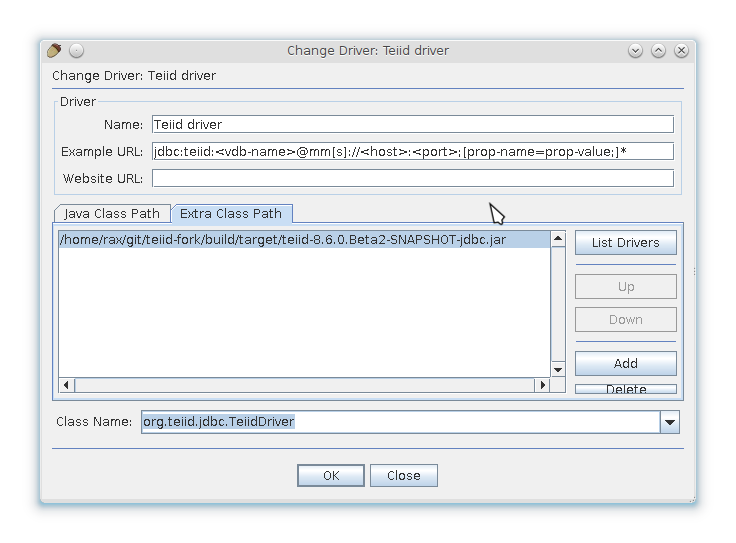
\includegraphics[scale=0.7]{driver}
 \label{driver}
 \caption{New driver settings}
\end{figure}
  
 \end{itemize}
\item Start Teiid
\begin{itemize}
 \item Start your application server like \texttt{bin/standalone.sh -c standalone-teiid.xml}
 \item If everything went right, something like \texttt{TEIID40003 VDB Test.1 is set to ACTIVE} should appear in application server log. This means, that virtual database is sucessfully deployed, connection to SimpleDB was successful and all metadata were loaded.
\end{itemize}
\item Connect Squirrell SQL client to running Teiid
\begin{itemize}
 \item Create new alias in Squirrel SQL Client
 \begin{itemize}
  \item As driver choose Teiid driver, created in step 2.
  \item URL is \texttt{jdbc:teiid:test@mm://localhost:31000}
  \item Default values for username and password are \texttt{user, user}
  \item Everything should look like on figure A.2. Now you can test the connection and save it. 
 \end{itemize}
 \begin{figure}[h]
 \centering
 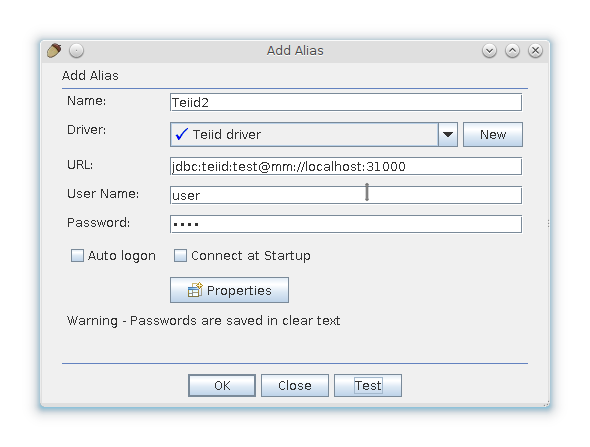
\includegraphics[scale=0.8]{newAlias}
 \caption{New alias settings}
 \end{figure}
\end{itemize}
\item Now you can try to execute SQL queries like:
\begin{itemize}
 \item \texttt{SELECT * FROM people WHERE director=true} for list of all directors
 \item or
 \begin{Verbatim}[fontsize=\small]
SELECT movies.title FROM movies 
 INNER JOIN people_movies 
    ON movies."itemName()"=people_movies.movieId 
 INNER JOIN people 
    ON people_movies.personId=people."itemName()" 
WHERE people.name='Emma Stone'
 \end{Verbatim}
for movie titles where Emma Stone was involved.
\item Let's try to add some movie:
 \begin{Verbatim}[fontsize=\small]
INSERT INTO movies 
  VALUES ('00021', '[Action;Comedy]', 
	  'My Studio', 'My novie', '5000')
 \end{Verbatim}
 Note here, that the second value will be stored as multivalued attribute. Format for working with multivalue attributes is semicolon separated values enclosed in brackets.
 \item Oh\dots Typo in movie title! Let's change that!
  \begin{Verbatim}[fontsize=\small]
UPDATE movies SET "title"='My movie' 
  WHERE "itemName()"='00021'
 \end{Verbatim}
 \item Want to delete movie from domain? No problem:
   \begin{Verbatim}[fontsize=\small]
DELETE FROM movies WHERE "itemName()"='00021'
 \end{Verbatim}
\end{itemize}


\end{enumerate}


\end{enumerate}

\chapter{Obsah přiloženého CD disku}
\begin{itemize}
 \item Složka \texttt{teiid-fork} s kompletními zdrojovými kódy projektu Teiid obsahující již změny provedené v rámci této práce.
 \item Soubor \texttt{teiidDiff} -- soubor obsahující všechny změny provedené v rámci této práce (výstup příkazu \texttt{git diff})
 \item Složka \texttt{importData} obsahující v sobě zdrojová data, projekt pro import dat do SimpleDB a soubor \texttt{README.md}, ve kterém je obsažen tutoriál
\end{itemize}


\end{document}
